\documentclass[11pt,ngerman]{scrartcl}

% standard packages
\usepackage[utf8]{inputenc}  % input in UTF-8
\usepackage[T1]{fontenc}  % output in T1 fonts (westeuropäische Codierung)
\usepackage{lmodern}  % latin modern fonts
\usepackage[ngerman]{babel}  % deutsches Sprachpaket, neue Rechtschreibung

% Seitensetup
\usepackage{scrlayer-scrpage}  % Seitenformatierung durch KOMA-interne Optionen
\usepackage[top=4cm, bottom=4cm]{geometry}  % Seitengeometrie (kann durch KOMA ersetzt werden, hab ich aber nicht geschafft)
\usepackage[hypcap=false]{caption, subcaption}  % caption editing - hypcap warning with hyperref
\usepackage{array}  % table editing

% additional packages
\usepackage{amsmath, amssymb, amstext}  % math packages (American Math Society)
\usepackage{bm}
\usepackage{icomma}  % Kommata in Dezimalzahlen verursachen keinen Abstand mehr
\usepackage{graphicx}  % Bilder einfügen
\usepackage{float} %Bilder placement
\usepackage{pdfpages}  % PDF als vollständige Seiten einfügen
\usepackage{lastpage}  % referenziert die letzte Seite
\usepackage[separate-uncertainty=true]{siunitx}  % bessere Darstellung von Einheiten
\usepackage{makecell} %Dicke Tabellenstriche
\usepackage{longtable}
\usepackage{booktabs}
%\usepackage{datatool}
\usepackage[hidelinks]{hyperref}  % hyperref verlinkt Referenzen - hidelinks entfernt borders um links

% package setups
% Kopf- und Fußzeile durch KOMA
\pagestyle{scrheadings}  % KOMA darf entscheiden
\clearpairofpagestyles  % reset
\setkomafont{pageheadfoot}{\normalfont}  % Standardschrift in Kopf- und Fußzeile
\captionsetup{format=plain, font=small, labelfont=bf} %Better caption, Abbildung ist FETT
%\setlength{\headheight}{27.2pt}  % benötigte Höhe Kopfzeile (warning von scrlayer-scrpage, wird aber automatisch so gerendert, falls diese Option weggelassen wird)
\ihead{Elastizität}  % Kopf links %Todo Titel ändern
\chead{\textsc{Philipp} Maximilian}  % Kopf Mitte %Todo Name ändern
\ohead{26 Mai 2021}  % Kopf rechts %Todo Datum ändern
\cfoot{\pagemark \, / \pageref{LastPage}}  % Fuß Mitte

% Table of Contents
\DeclareTOCStyleEntry{dottedtocline}{section}  % KOMA intern - Inhaltsverzeichnis mit Punkten (nur sections)

%Overbar setup
\newcommand{\overbar}[1]{\mkern 1.5mu\overline{\mkern-1.5mu#1\mkern-1.5mu}\mkern 1.5mu}
% SI
\sisetup{locale = DE}  % deutschsprachige SI-Konvention
\sisetup{quotient-mode = fraction}
\sisetup{per-mode = fraction}
\DeclareSIUnit\px{px}

% citation
\usepackage{csquotes}
\usepackage[backend=biber]{biblatex}
\addbibresource{elastizitat.bib} %Todo .bib befüllen zb.: mit JabRef (Empfehlung der Redaktion)

% array
\renewcommand{\arraystretch}{1.2}

\begin{document}

%
\includepdf{pdfs/Deckblatt.pdf} % Todo Deckblatt ausfüllen
\title{Elastizität}
\author{\textsc{Philipp} Maximilian\\11839611}
\date{26.05.2021}
\maketitle

\tableofcontents
\newpage
\section{Aufgabenstellung}
\label{sec:aufgabenstellung} 

\begin{enumerate}
    \item Wiegen der Gewichte des Gewichtssatzes, messen des Abstands
        der Auflageschneiden mit einem Maßband und die Bestimmung der Stababmessungen (Höhe,
        Breite, Länge bzw.  Durchmesser) mit einer Schiebelehre.
    \item Ermittlung des Flächenträgheitsmoments durch die Messungen für ein vorgegebenes Stabprofil.
    \item Bestimmung der maximale Durchbiegung
    \item Bestimmung des Elastizitätsmodul E eines Stabes, anhand seiner Durchbiegung
    \item Wiederholung des Biegeversuchs mit einem anderen Material
\end{enumerate}

\section{Voraussetzungen und Grundlagen} \label{sec:voraussetzungen_grundlagen}
Folgende Grundlagen wurden aus dem zur Verfügung gestellten Vorlagen
\cite{vorlageelast1} \cite{vorlageelast2}  und dem Mechanik Vorlesungskript \cite{Knoll2020}
entnommen und für dieses Experiment leicht angepasst.

Wirken auf einen Körper äußere Kräfte, die im Gleichgewicht sind, so tritt eine
Änderung der Form und des Volumens des Körpers ein, die bei Beenden der
Kraftwirkung wieder vollständig zurückgeht, solange die Deformation die Grenze
des elastischen Bereiches nicht überschreitet. Die Dehnung $\varepsilon$
(positiv oder negativ) ist dann proportional der wirkenden Spannung $\sigma$.
Die Proportionalitätskonstante $E$ wird Elastizitätsmodul genannt. Dieser
Zusammenhang ist in Gleichung \ref{eq:Dehnung_Spannung} dargestellt.

\begin{equation}
    \label{eq:Dehnung_Spannung}
    \sigma = \frac{F}{A} = E\frac{\Delta l}{l} = \varepsilon E
\end{equation}

Betrachtet man einen Balken oder Stab, welcher zwischen zwei Punkten im Abstand
$L$ gelagert ist und auf welchen in der Mitte eine Kraft $F$ wirkt, kommt es zu
einer Durchbiegung.  Dabei lässt sich die maximale Durchbiegung $w_{max}$ bei
kleinen Durchbiegungen mittels Gleichung \ref{eq:max_Durchbiegung} beschreiben.

\begin{equation}
    \label{eq:max_Durchbiegung}
    w_{max} = \frac{FL^3}{48EI_y}
\end{equation}

$I_y$ beschreibt hierbei das Flächenträgheitsmoment des Stabes: 
\begin{align}
    I_y &= \int z^2 \text{d}A \\
    I_y &= \frac{bh^3}{12} \quad  \text{für rechteckiges Stabprofil}  \label{eq:Flaechentraegheitsmoment_Rechteck} \\
    I_y &= \frac{\pi d^4}{64}  \quad \text{für kreisförmiges Stabprofil} \label{eq:Flaechentraegheitsmoment_Kreis} \\
\end{align}

Wobei $z$ der senkrechte Abstand der y-Achse zum $\text{d}A$ Element ist. $b$ ist die 
Dicke und $h$ die Höhe des rechteckigen Stabes. $d$ ist der Durchmesser
des runden Stabes.

Die maximale Biegespannung $\sigma_{max}$ lässt sich durch das, durch die Kraft 
enstandene, Biegemoment $M_b$, der Stabhöhe $h$ und dem Flächenträgheitsmoment $I_y$
anschreiben:
\begin{equation}
    \label{eq:Spannung_max}
    \sigma_{max} = \frac{hM^{max}_b}{2I_y}
\end{equation}
Das maximale Biegemoment ist, wie zuvor erwähnt, abhängig von der Kraft $F$ und
der Länge $L$ des Stabes, die \autoref{eq:Biegemoment} zeigt diesen Zusammenhang:

\begin{equation}
    \label{eq:Biegemoment}
    M_{max} = \frac{FL}{4} = \frac{mgL}{4}
\end{equation}

Um zu sehen, wie sich die Unsicherheit der Messungen bis in die Ergebnisse 
fortpflanzt, ist \autoref{eq:Unsicherheitsfortpflanzung} verwendet worden.
Die Grundlagen dieser Gleichung sind von den Powerpointfolien von 
GUM entnommen worden.\cite{WolfgangKessel2004} Die Verallgemeinerung ist von Wikipedia entnommen
worden \cite{2020Fehler}.
Für die Auswertung ist die Progammiersprache Python im speziellen das 
Packet \verb#scipy#, zur Hilfe genommen worden.

\begin{equation}
    \label{eq:Unsicherheitsfortpflanzung}
    V_y = J(x) \cdot V_x \cdot J^{T}(x)
\end{equation}

Wobei $V_y$ und $V_x$ die Kovarianzmatrizen von den Vektoren $\bm{y}$ und $\bm{x}$ sind.
$\bm{x}$ ist der Vektor der Eingangsvariablen und $\bm{y}$ ist der Vektor der Ausgangsvariablen.
$J$ ist die Jakobimatrix der vektorwertigen Funktion $\bm{y} = \vec{F}(\bm{x})$ ist.
So lassen sich die Komponenten der Matrix relativ einfach anschreiben $J_{ij}(x) = \frac{\partial{y_i}}{\partial{x_j}}(x)$.
Damit man die Unsicherheit der einzelnen Variablen $y_i$ bekommt, muss nur die Quadratwurzel des i-ten Diagonalelementes der 
$\bm{y}$-Kovarianzmatrix genommen werden $u_i= \sqrt{\mathrm{diag}(V_y)_i}$.
Da in diesem Experiment meistens nur skalare Funktionen untersucht werden, vereinfacht
sich die \autoref{eq:Unsicherheitsfortpflanzung} dramatisch und die Unsicherheit
der Variable $y$ lässt sich einfach so berechnen:

\begin{equation}
    \label{eq:graduncentainty}
    u_y = \sqrt{\mathrm{grad} y^T \cdot V_x \cdot \mathrm{grad} y}
\end{equation}

\section{Versuchsanordnung}
\label{sec:versuchsanordnung}
Zwei Sessel werden einander gegenüber gestellt und der zu untersuchende Stab
hinaufgelegt, siehe \autoref{fig:aufbau}. Weiters wird ein dritter Sessel
benötigt um einen Schuhlöffel als Referenzpunkt mit
Panzerband dort zu befestigen, siehe
\autoref{fig:schuhloffel}. Alle Messungen werden von diesem Referenzpunkt aus
gemacht.

\begin{figure}[H]
    \centering
    \begin{minipage}[htbp]{\linewidth}
        \begin{minipage}[htbp]{.45\linewidth} % [b] => Ausrichtung an \caption
            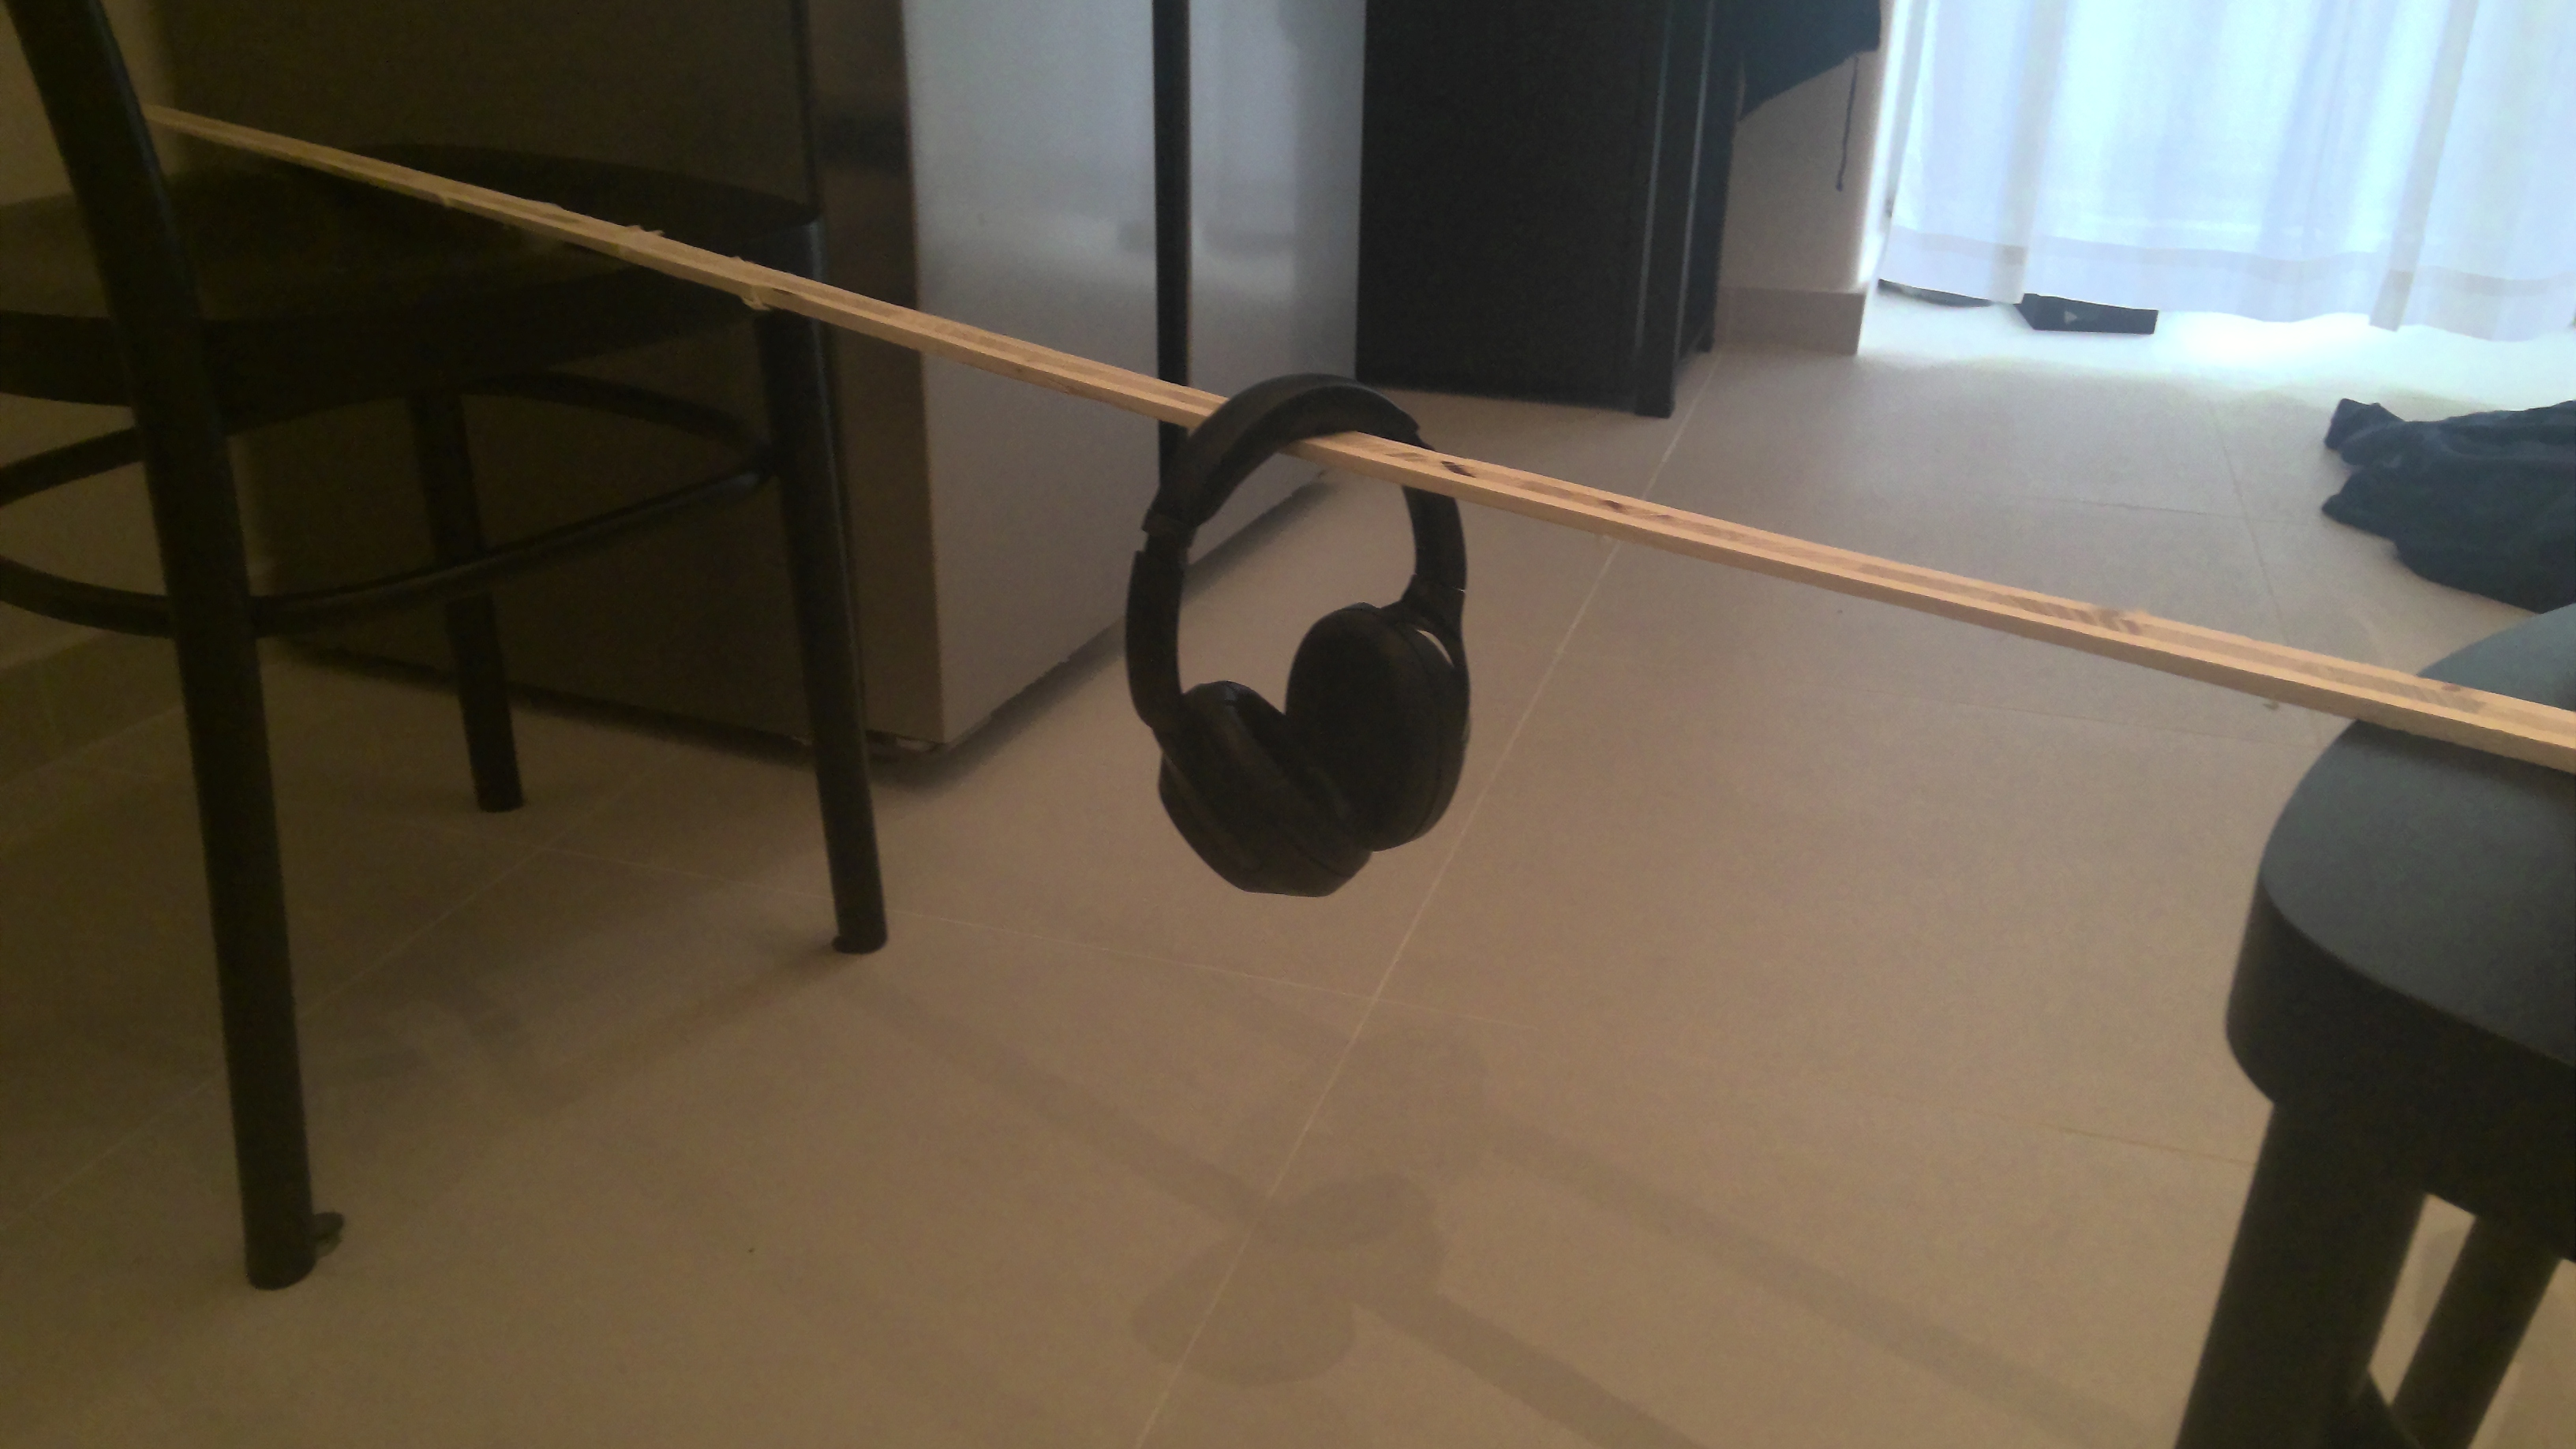
\includegraphics[width=\linewidth]{pics/aufbau1.jpg}
        \caption[Aufbau des Experiments]{Aufbau des Experiments wo der Träger
        zwischen den zwei Sesseln belastest wird.}
        \label{fig:aufbau}
        \end{minipage}
        \begin{minipage}[htbp]{.50\linewidth} % [b] => Ausrichtung an \caption
            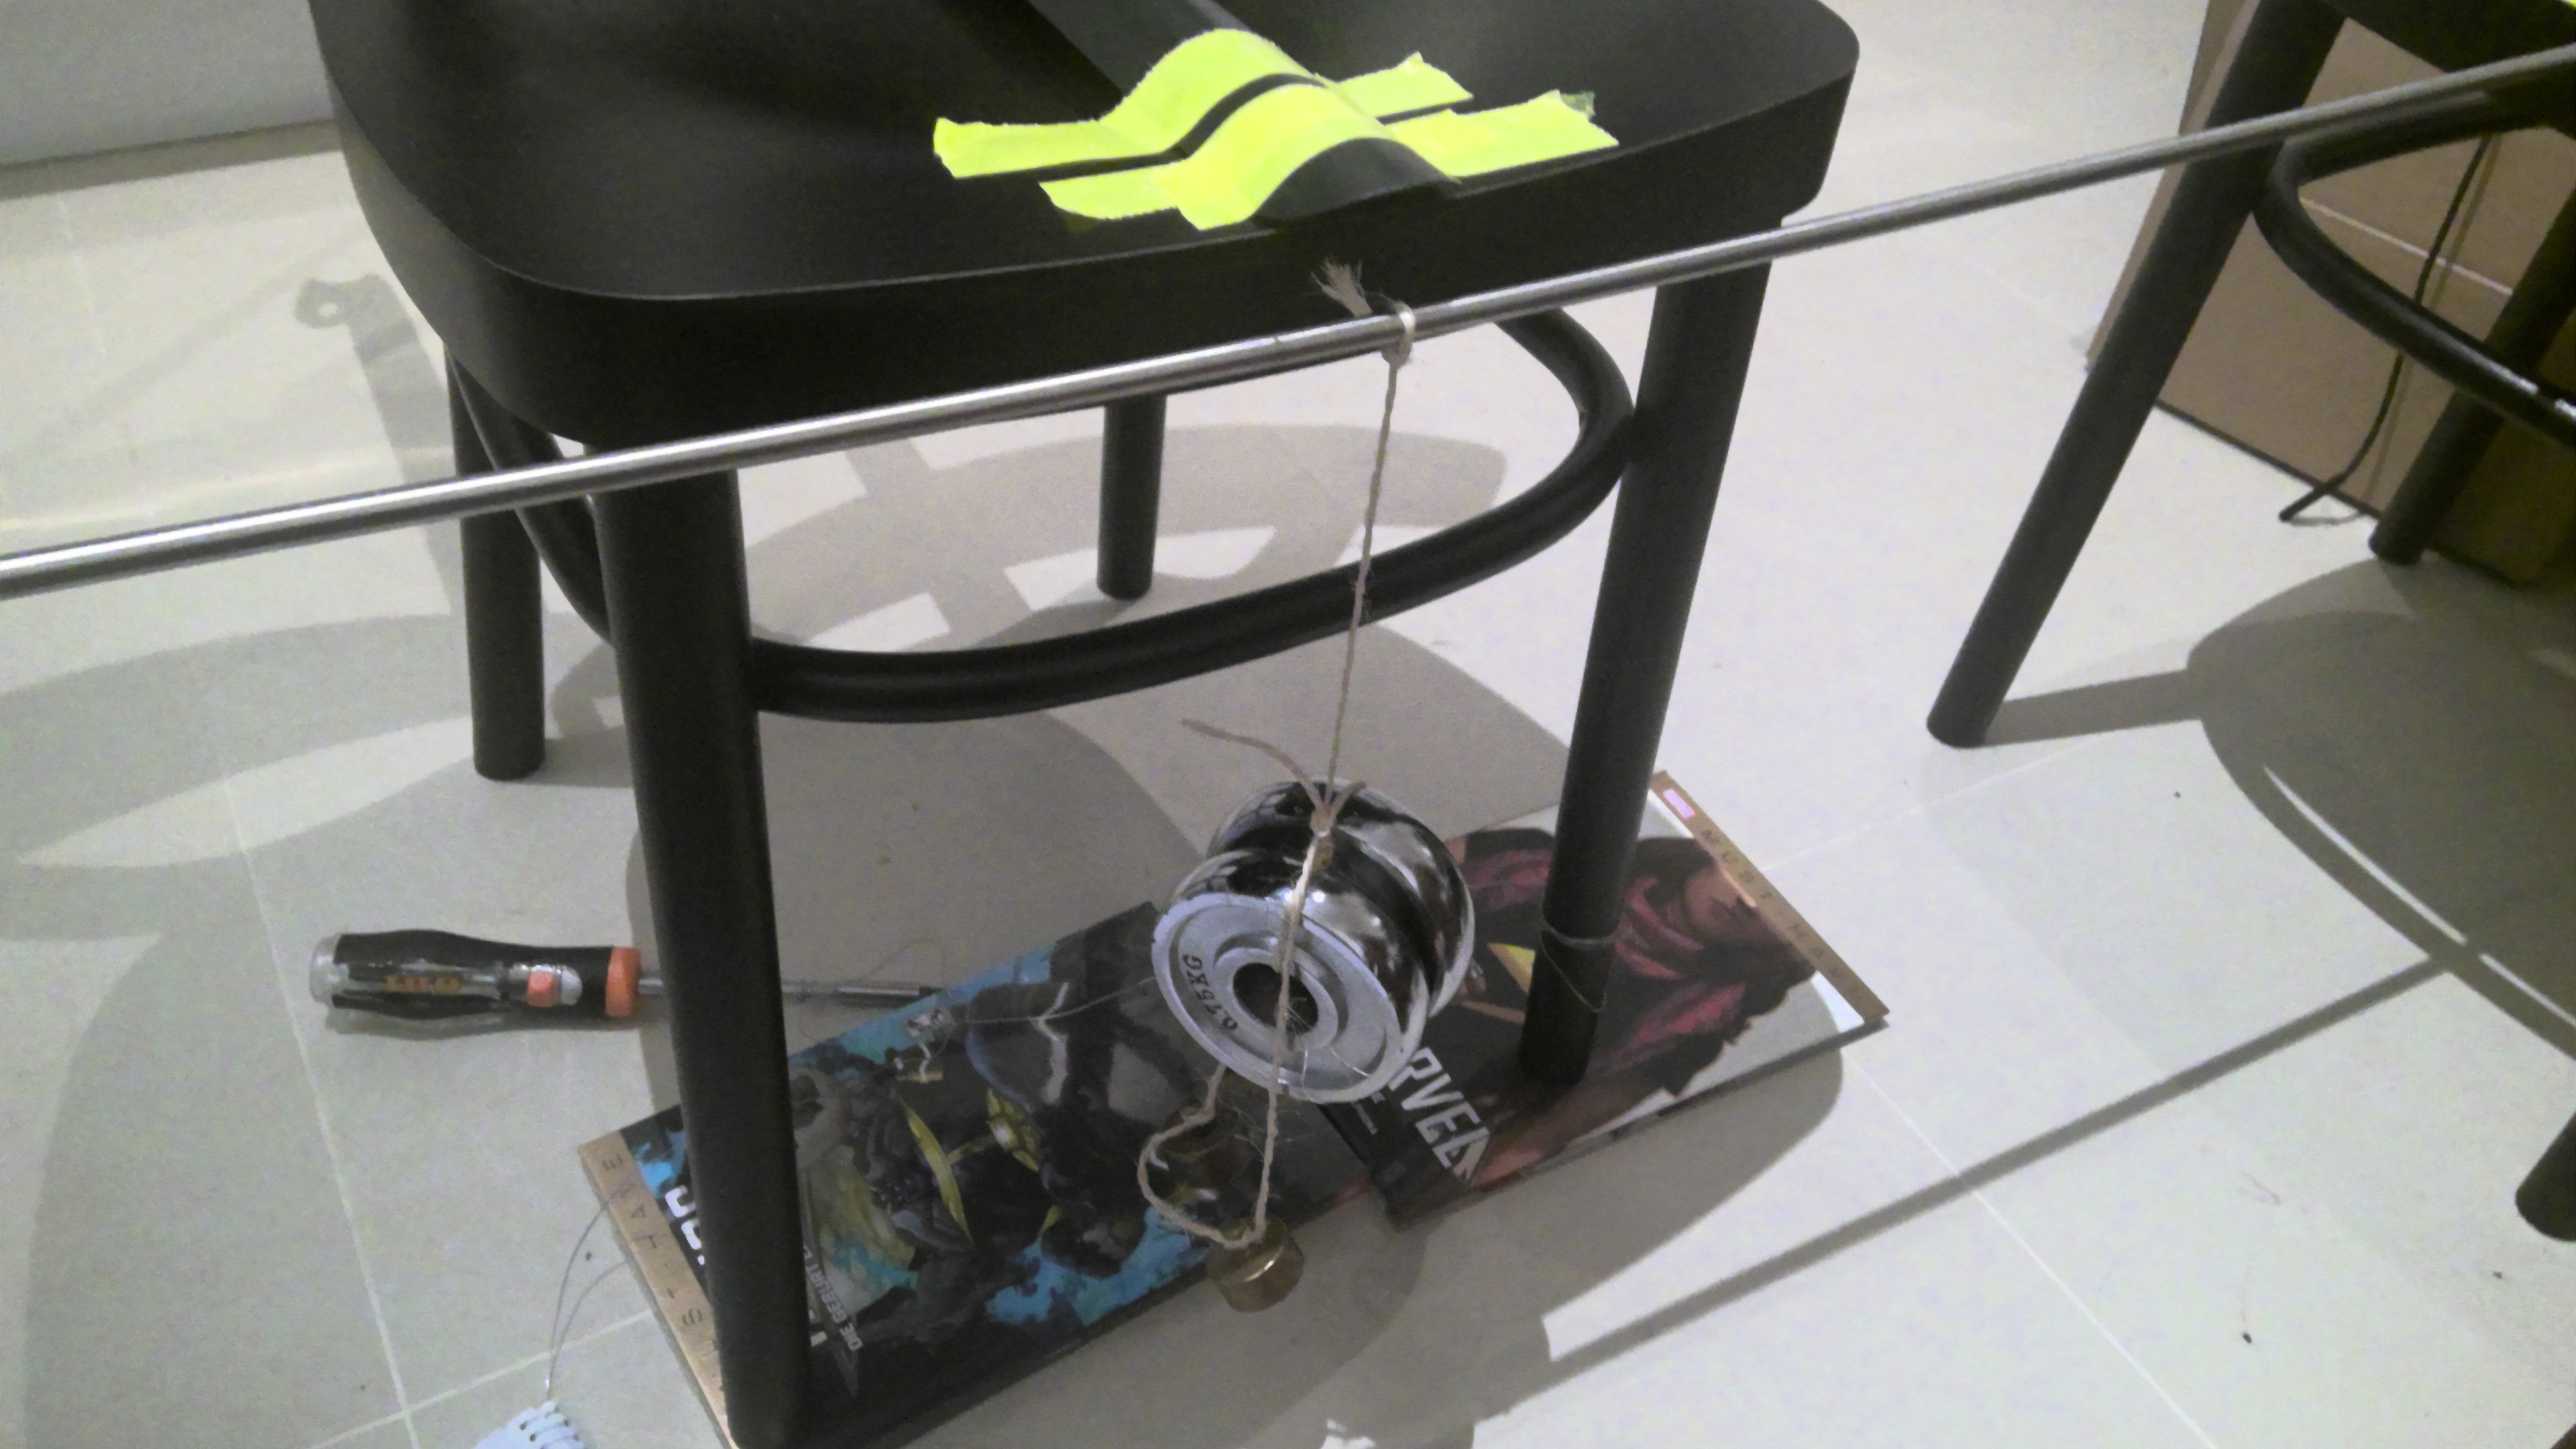
\includegraphics[width=\linewidth]{pics/aufbau2.jpg}
        \caption[Aufbau des Experiments Schuhlöffel]{Aufbau des Referenzpunkts}
        \label{fig:schuhloffel}
        \end{minipage}
    \end{minipage}
 \end{figure}


\section{Geräteliste}
\label{sec:geraeteliste}
%\setlength\LTleft{-6.5em}
\begin{longtable}{c|c|S|p{15em}}
\caption[Geräteliste]{Verwendete Geräte \label{tab:geraeteliste}} \\  % optionales Argument wird in Verzeichnissen verwendet, essentielles Argument direkt im Text
\toprule
Gerät                              & Gerät-Nr. & { Unsicherheit }  & Bemerkungen \\  
\midrule
\endfirsthead
\caption[]{(Fortsetzung)}\\
\toprule
Gerät                              & Gerät-Nr. & { Unsicherheit }  & Bemerkungen \\                                                                        
\midrule
\endhead
\endfoot
\endlastfoot
        Holzstab, eckig & axx & \SI{3}{\ms}       & Objekt von dem das E-Modul bestimmt wird\\ \hline
        Maßband         & bxx & \SI{1}{\mm}       & Um die Länge bzw. den Überhang der Stäbe zu messen \\ \hline
        Schublehre      & cxx & \SI{0.02}{\mm}    & Um die Dicke bzw. Höhe der Stäbe zu messen \\ \hline
        Stahlstab, rund & dxx & { - }             & Für die Bestimmung des E-Moduls eines anderes Materials \\ \hline
        Stühle 3x       & fxx & { - }             & Dienen als Loslager für die Träger \\ \hline
        Schuhlöffel     & hxx & { - }             & Dient als Referenzpunkt \\ \hline
        Panzerband      & ixx & { - }             & Um den Schuhlöffel fest an einem Stuhl zu befestigen\\ \hline
        Set-Präzision Gewichte     & jxx & \SI{+-0.02}{\gram} & Eichung Österreichischeseichamt \\ \hline
        \SI{0.75}{\kg} Gewichte 2x & kxx & \SI{+-10}{\gram} & Gewogen mit Waage die eine Unsicherheit von \SI{+-3}{\g}@\SI{0.75}{\kg} \\ \hline

        \hline
\end{longtable}

\section{Versuchsdurchführung und Messergebnisse}
\label{sec:versuchsdurchfuehrung_messergebnisse}
Für die Biegeversuche werden die Stäbe auf zwei Sessel gelegt. Im nächsten
Schritt werden in der Mitte der Stäbe Gewichte fixiert, bis eine gewisse
Deformation des Stabes erkenntlich ist, wodurch sich das E-Modul bestimmen
lässt. Dies wird mit verschiedenen Gewichten gemacht um ein Reihe an Messwerten 
zu bekommen. Dieser Versuch wird für die verschiedenen Materialien wiederholt. 
Dies wurde mit einem rechteckigen Holzstab und einem runden Stahlstab durchgeführt.
In folgenden Tabellen sind die erhaltenen Auslenkungen bei einem bestimmten
Gewicht aufgelistet:

\begin{table}[H]
    \centering
    \caption{
        Diese Tabelle beinhaltet die Gewichte $m_i$ und die Auslenkung $\omega_{max_{i}}$,
        die die entsprechenden Gewichte bei einem Holzstab verursachen:\\
        $m_{i}$ ist die Aufgehängte Masse \\
        $\omega_{max_{i}}$ ist die, durch die Masse verursachte, Deflektion vom Referenzpunkt aus \\
        ref ist die Distanz vom Referenzpunkt zum Messpunkt bei keinem Gewicht \\
    }
    \label{tab:messwerte_holz}
    \begin{tabular}{l|S|S|S|S}
        i   & {$m_i$}     & {$\Delta m_i$} & $\omega_{max_{i}}$ & $\Delta \omega_{max_{i}}$ \\
        {}  & {/ \si{\g}} & {/ \si{\mg}}    & {/ \si{\cm}}       & {/ \si{\cm}} \\ \hline \hline
        ref & 0   & 0   & 0.912 & 0.02\\
        1   & 20  & +-2 & 1.028 & 0.02\\
        2   & 50  & +-2 & 1.252 & 0.02\\
        3   & 70  & +-2 & 1.514 & 0.02\\
        4   & 100 & +-2 & 1.710 & 0.02\\
        5   & 120 & +-2 & 1.936 & 0.02\\
        6   & 150 & +-2 & 2.158 & 0.02\\
        7   & 200 & +-2 & 2.578 & 0.02\\
        8   & 220 & +-2 & 2.716 & 0.02\\
        9   & 250 & +-2 & 2.922 & 0.02\\
        10  & 270 & +-2 & 3.122 & 0.02\\
        11  & 300 & +-2 & 3.342 & 0.02\\
        12  & 320 & +-2 & 3.502 & 0.02\\
        13  & 350 & +-2 & 3.706 & 0.02\\
        14  & 400 & +-2 & 4.088 & 0.02\\
    \end{tabular}
\end{table}


\begin{table}[H]
    \centering
    \caption{
        Diese Tabelle beinhaltet die Gewichte $m_i$ und die Auslenkung $\omega_{max_{i}}$,
        die die entsprechenden Gewichte bei einem Stahlstab verursachen:\\
        $m_{i}$ ist die Aufgehängte Masse \\
        $\omega_{max_{i}}$ ist die, durch die Masse verursachte, Deflektion vom Referenzpunkt aus \\
        ref ist die Distanz vom Referenzpunkt zum Messpunkt bei keinem Gewicht \\
    }
    \label{tab:messwerte_stahl}
    \begin{tabular}{l|S|S|S|S}
        i   & {$m_i$}     & {$\Delta m_i$} & $\omega_{max_{i}}$ & $\Delta \omega_{max_{i}}$ \\
        {}  & {/ \si{\g}} & {/ \si{\g}}    & {/ \si{\cm}}       & {/ \si{\cm}} \\ \hline \hline
        ref & 0    & 0      & 1.820 & 0.02\\
        1   & 200  & +-0.02 & 1.912 & 0.02\\
        2   & 400  & +-0.02 & 2.042 & 0.02\\
        3   & 750  & +-10   & 2.246 & 0.02\\
        4   & 1150 & +-10   & 2.536 & 0.02\\
        5   & 1500 & +-20   & 2.706 & 0.02\\
        6   & 1700 & +-20   & 2.778 & 0.02\\
        7   & 1900 & +-20   & 2.958 & 0.02\\
    \end{tabular}
\end{table}

Das exakte Ablesen der Werte war schwierig, deshalb sind die Unsicherheiten bei der Längenmessung
deutlich höher, im Vergleich zur Genauigkeit der Schublehre.


Die Länge von Lager zu Lager wurde auch bestimmt:

\begin{table}[H]
    \centering
    \caption{
        Diese Tabelle beinhaltet die Distanz von Lager zu Lager der
        zwei Messungen. \\
        $L_{Holz}$ ist die Distanz von Lager zu Lager bei der Messung vom Holz\\
        $L_{Stahl}$ ist die Distanz von Lager zu Lager bei der Messung vom Stahl\\
    }
    \label{tab:L}
    \begin{tabular}{l|S|S}
        Symbol                 & {Werte}     & {$\Delta$} \\ \hline \hline
        $L_{Holz}$ / \si{\cm}  & 119 & +-0.1\\ 
        $L_{Stahl}$ / \si{\cm} & 100 & +-0.1\\
    \end{tabular}
\end{table}

Die Dimensionen des Holzstabes sind die Breite $b$ = \SI{2.60(7)}{\cm} und die Höhe $h$
= \SI{6.7(7)}{\mm} 
da der Holzstab über die Länge variiert, konnten
diese Werte nicht genauer bestimmt werden.

Der Durchmesser des runden Stahlstabes ist \SI{8.00(2)}{\mm}.

\section{Auswertung}
\label{sec:auswertung}

Zunächst lässt sich das Flächenträgheitsmoment vom rechteckigen Holzstab
$I_{H}$ \autoref{eq:Flaechentraegheitsmoment_Rechteck} und dann das
Flächenträgheitsmoment vom runden Stahlstab $I_{S}$
\autoref{eq:Flaechentraegheitsmoment_Kreis} bestimmen:

\begin{equation}
    I_H = \SI{7(3)e-10}{\meter\tothe{4}}
\end{equation}

\begin{equation}
    I_S = \SI{2.01(3)e-10}{\meter\tothe{4}}
\end{equation}

Formt man \autoref{eq:Biegemoment} nach $E$ um und nimmt die Kraft $F=mg$ gleich
der Gravitationskraft, wobei $m$ die Masse der Objekte und $g$ = \SI{9.81}{\meter\per\second\squared}
die Erdbeschleunigung ist, können die Werte aus \autoref{tab:messwerte_holz} \ref{tab:messwerte_stahl}
\ref{tab:L} genommen werden um eine Reihe an Werten für das E-Modul zu bekommen.

\begin{equation}
    E = \frac{g L^3}{48\omega_{max}I_y} m 
\end{equation}

Wenn diese Werte nun gemittelt werden und der Standarderror davon berechnet wird,
bekommt man folgende Werte für das E-Modul von Stahl $E_S$

\begin{equation}
    E_S = \SI{181(8)}{\GPa}
\end{equation}

und für das E-Modul von Holz

\begin{equation}
    E_S = \SI{6(5)}{\GPa}
\end{equation}

Eine andere Methode wäre das E-Modul mittels einem linearen Fit zu finden
indem man die maximale Deflektion $\omega_{max}$ über das belastende Gewicht
$m$ aufträgt.

\begin{equation}
    \omega_{max} = \frac{g L^3}{48 E I_y} m  \label{eq:linreg}
\end{equation}


\begin{figure}[H]
    \centering
    \begin{minipage}[htbp]{\linewidth}
        \begin{minipage}[htbp]{.48\linewidth} % [b] => Ausrichtung an \caption
            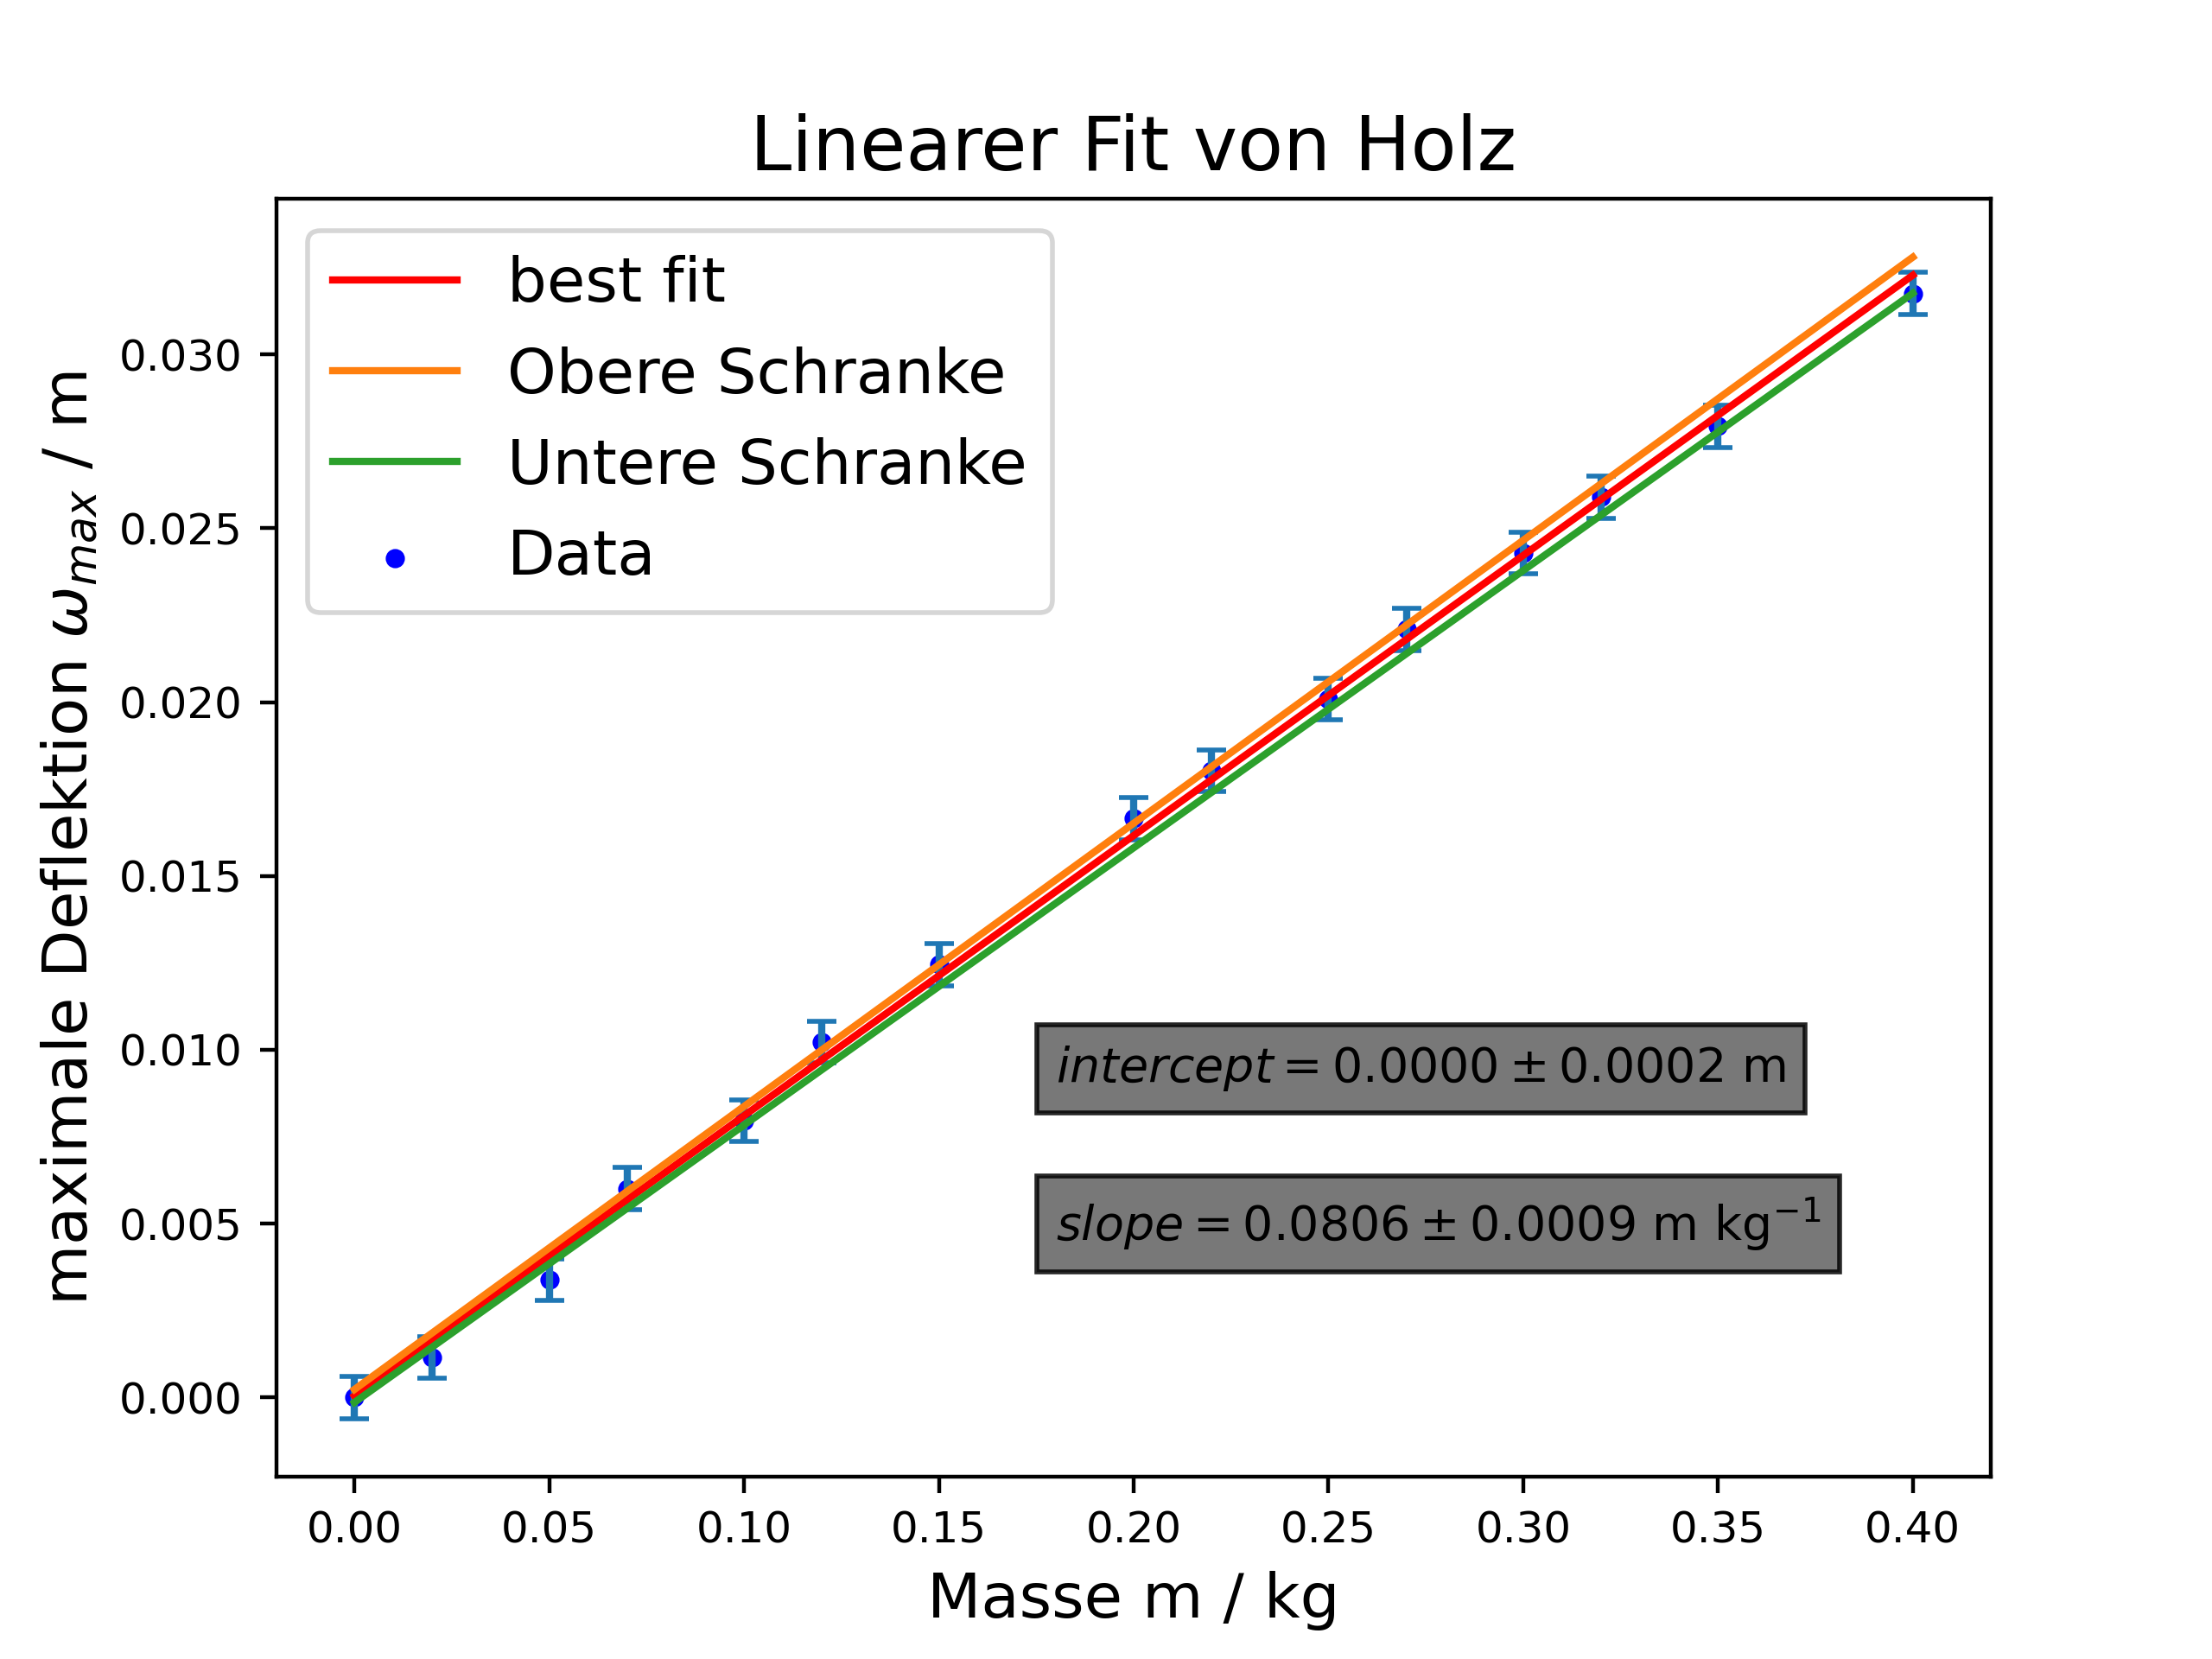
\includegraphics[width=\linewidth]{pics/fit/lin_reg_m_w_messreihe_1.png}
            \caption[Linearer-Fit Holz]{Die Daten aus \autoref{tab:messwerte_holz}
            an diese \autoref{eq:linreg} gefittet um die Steigung zu bestimmen, mit der dann das E-Modul von Holz gefunden werden kann.}
            \label{fig:linregholz}
        \end{minipage}
        \begin{minipage}[htbp]{.48\linewidth} % [b] => Ausrichtung an \caption
            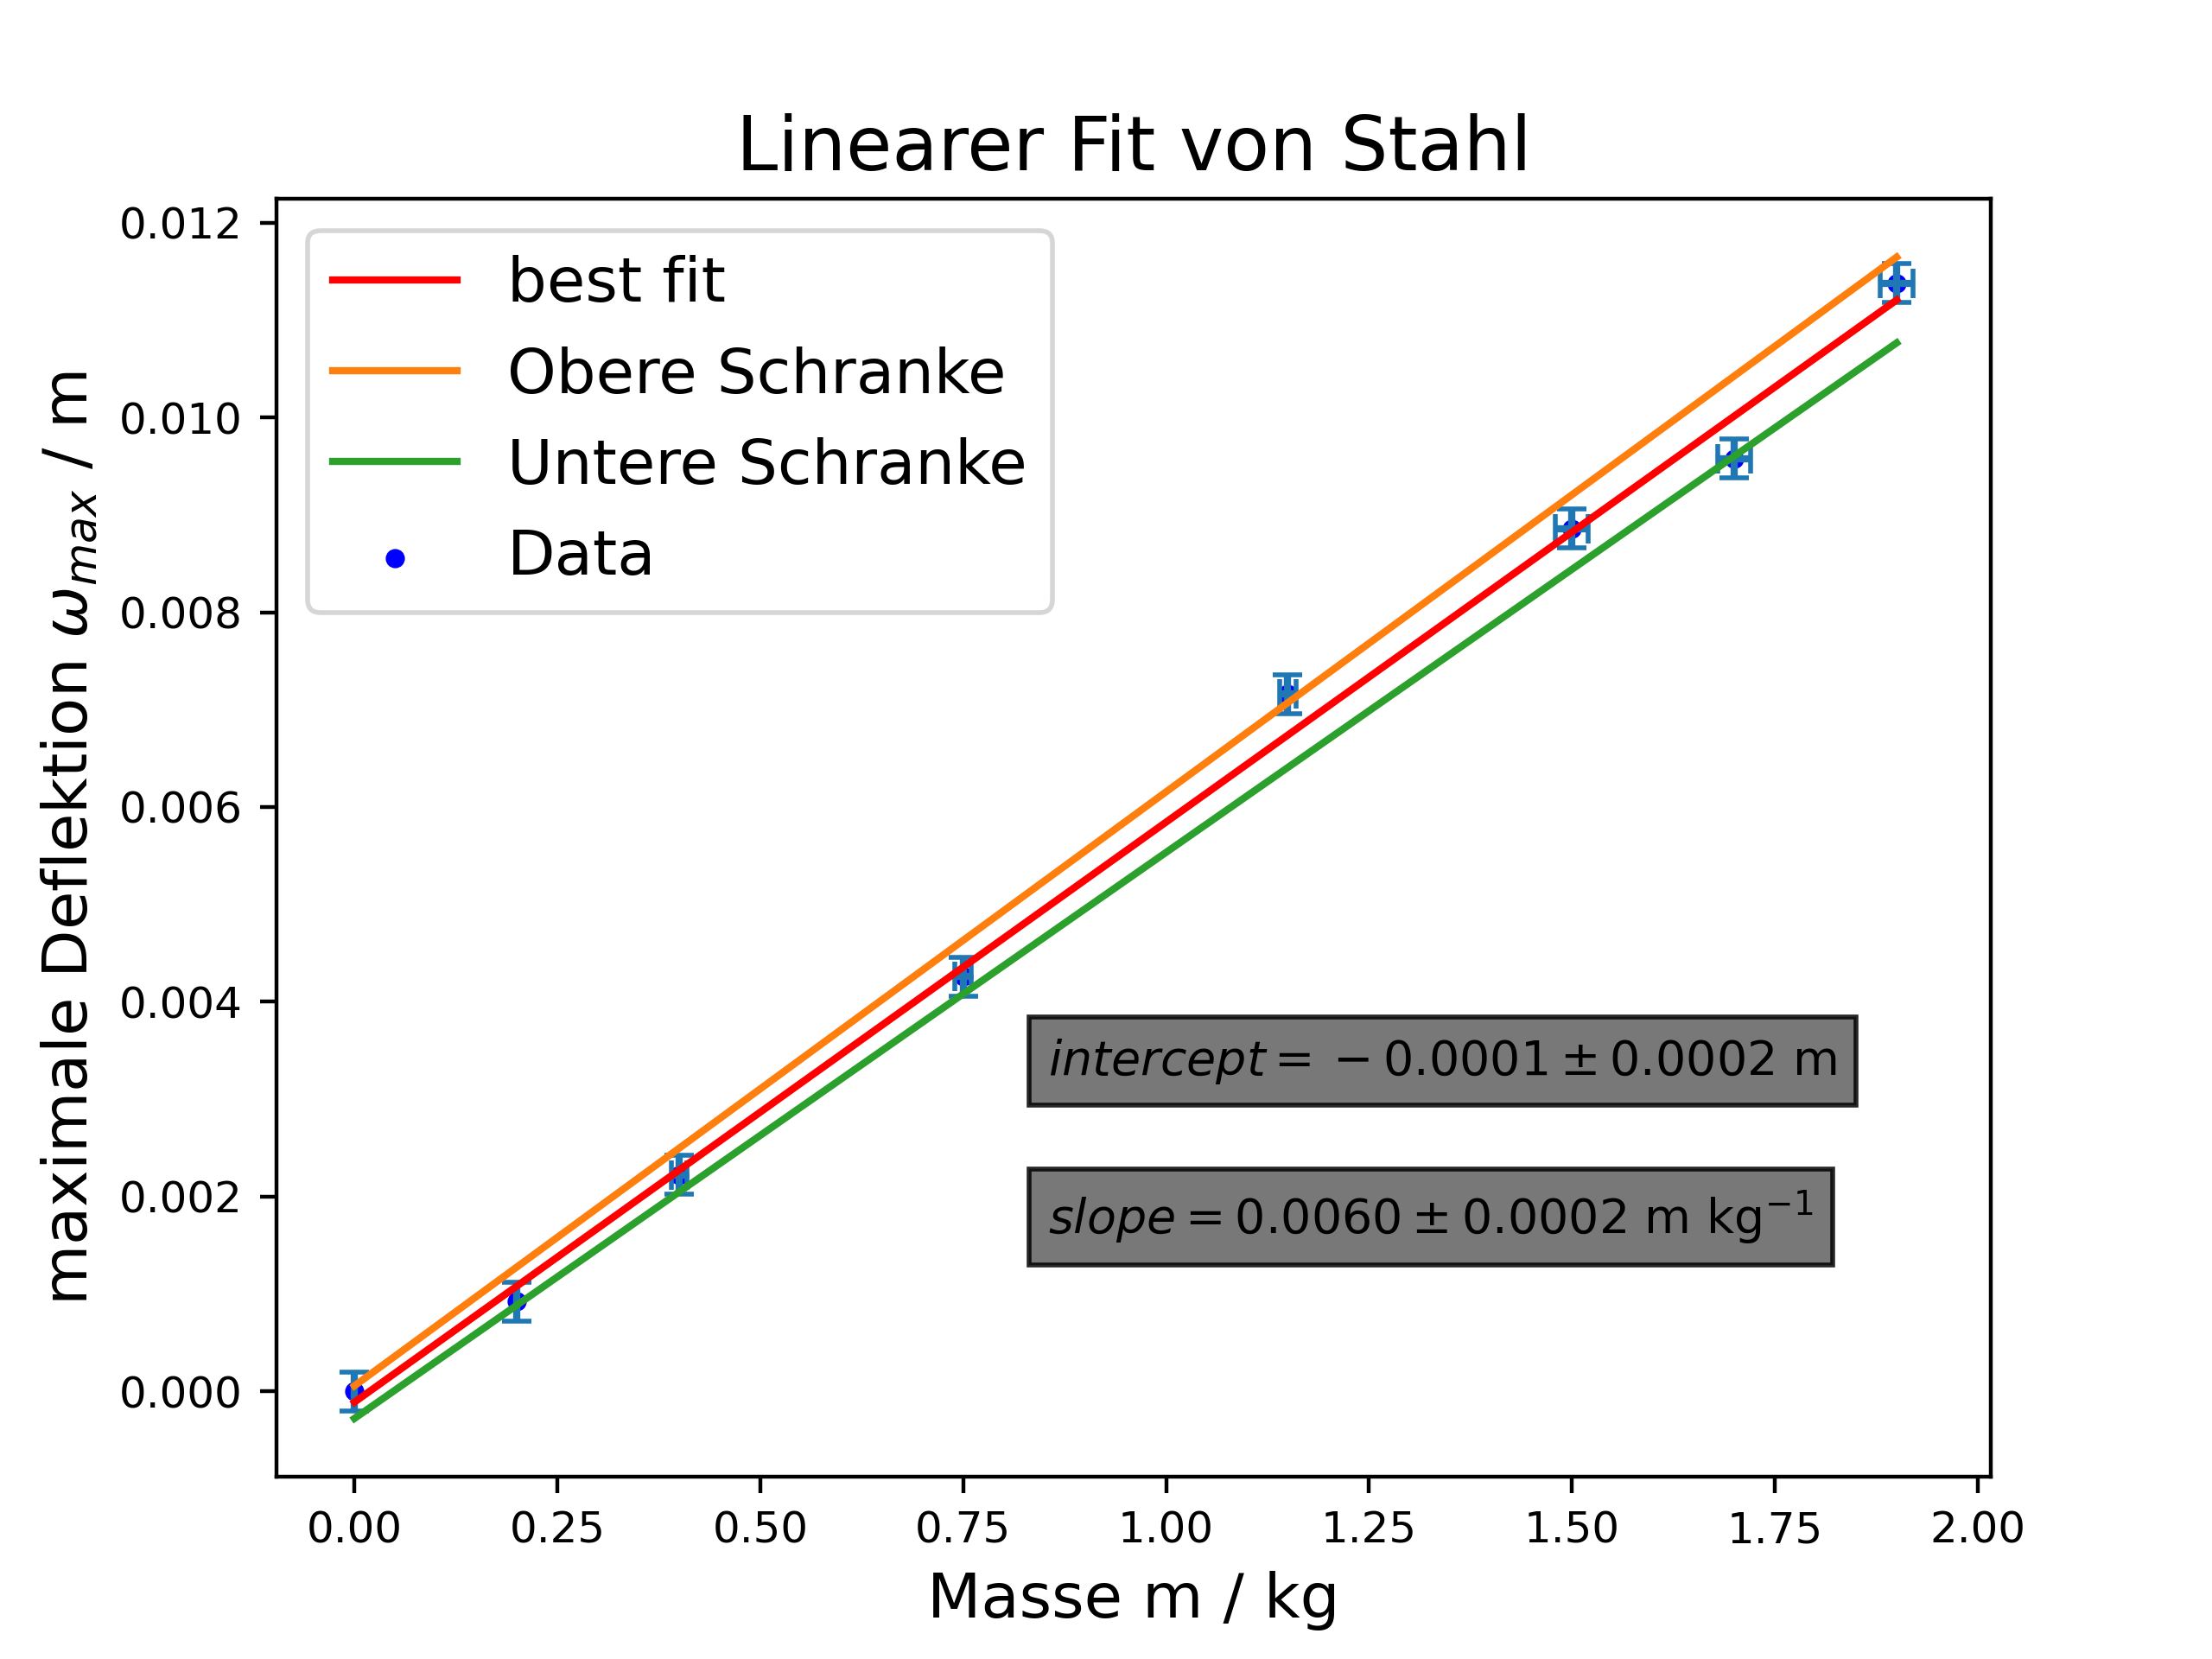
\includegraphics[width=\linewidth]{pics/fit/lin_reg_m_w_messreihe_2.png}
        \caption[Linearer-Fit Stahl]{Die Daten aus \autoref{tab:messwerte_stahl}
            an diese \autoref{eq:linreg} gefittet um die Steigung zu bestimmen,
            mit der dann das E-Modul von Stahl gefunden werden kann. }
            \label{fig:linregstahl}
        \end{minipage}
    \end{minipage}
\end{figure}


Vergleicht man die durch das Fitten erhaltene Steigung (slope) $k$
mit der Steigung der \autoref{eq:linreg}, so ergibt sich ein Wert für
das E-Modul.

So erhält man für Stahl einen Wert von
\begin{equation}
    E_S = \SI{170(60)}{\GPa}
\end{equation}
und für Holz einen Wert von
\begin{equation}
    E_H = \SI{6(5)}{\GPa}
\end{equation}

\section{Diskussion und Zusammenfassung}
\label{sec:diskussion_zusammenfassung}
% Aufzählung was scheiße glaufen is

Nun werden die verwendeten Methoden diskutiert und die Ergebnisse 
zusammengefasst.

Die erhaltenen Werte aus dem Kapitel \nameref{sec:auswertung} 
für die E-Module von Stahl $E_S$ und Holz $E_H$ beinhalten
die Literaturwerte, siehe \autoref{tab:ergebnisse} jedoch sind die relativen Unsicherheiten
überwiegend groß, wodurch nicht wirklich eine Aussage getroffen werden kann.

\begin{table}[H]
    \centering
    \caption{Messergebnisse für das E-Modul für Stahl und Holz, unter Verwendung
    von einem Linearen-Fit und dem Mittel von mehreren Messungen. Zudem
    die Gegenüberstellung von den Messwerten zu den Literaturwerten}
    \label{tab:ergebnisse}
    \begin{tabular}{c|S|S|S}
        $E$ / GPa & {Mittelung} & {Linearer Fit} & {Literaturwert} \\ \hline
        Holz & 6(5) & 6(5) & \numrange{10}{15} \cite{wikielasti2021} \\
        Stahl & 181(8) & 170(60) & \numrange{180}{210} \cite{Ahrberg2011} \\ 
    \end{tabular}
\end{table}

Der einzige brauchbare Wert ist der Wert für das E-Modul von Stahl,
welcher durch Mittelung der Messwerte bestimmt wurde.

Verbesserungsvorschläge sind:

\begin{enumerate}
    \item Einen besseren Holzstab nehmen, da dieser nicht wirklich
        perfekt homogen war.
    \item Mehrere Messungen des Holzstabes mit größeren Gewichtsabständen
    \item Verwendung von genaueren und schwereren Gewichten
\end{enumerate}

Dieses Experiment, war um es kurz zu fassen, ein experimentalphysikalisches
Weihefestspiel (indirektes Zitat Helmuth Mayr BWB2 2019).

Eine gute Sache, welche noch zu erwähnen wäre, ist, dass der Referenzpunkt mit
dem Schuhlöffel sehr gut funktioniert hat. So sollte es immer gemacht werden.




% Literaturtabelle
\newpage
\printbibliography

\listoffigures

\listoftables


\end{document}
